\documentclass[9pt]{beamer}

\usetheme{TUDo}



% Encoding je nach Compiler
\ifluatex
\usepackage[utf8]{luainputenc}
\else
\usepackage[utf8]{inputenc}
\usepackage[T1]{fontenc}
\fi

%Links
\usepackage[]{hyperref}


\renewcommand{\figurename}{Fig.}

%%%%%%%%%%%%%%%%%%%%%%%%%%%%%%%%%%%%%%%%%%%%%%%%%%%%%%%%%%%%%%%%%%%%%%%%%%%%%%%%
%%%%%-------------Hier Titel/Autor/Grafik/Lehrstuhl eintragen--------------%%%%%
%%%%%%%%%%%%%%%%%%%%%%%%%%%%%%%%%%%%%%%%%%%%%%%%%%%%%%%%%%%%%%%%%%%%%%%%%%%%%%%%

\title{Wordspotting von segmentierten Dokumentenabbildern}
\author{Stephan Abel, Ivan Danov, Simon Demming}
\institute[]{\par\smallskip\smallskip Faculty for Computer Science}


\begin{document}

	\begin{frame}
		\setcounter{framenumber}{0}
	    \titlepage
	\end{frame}
	
	\section{Einführung}
	
		\subsection{Die Aufgabe}
			
			\begin{frame}
				\frametitle{Die Aufgabe}
				Wordspotting mit segmentierten Dokumentenabbildern\\
				Inverted File Structure\\
				Spatial Pyramid\\
			\end{frame}
			
		\subsection{Vorbereitungen}
		
			\begin{frame}
				\frametitle{Vorbereitungen}
				Ground Truth verarbeiten\\
				Deskriptoren berechnen\\
				Clustern -> Codebook berechnen\\
			\end{frame}
			
	\section{Durchführung}
	
		\subsection{Ground Truth}
			
			\begin{frame}
				\frametitle{Ground Truth}
				\begin{figure}
					\centering
					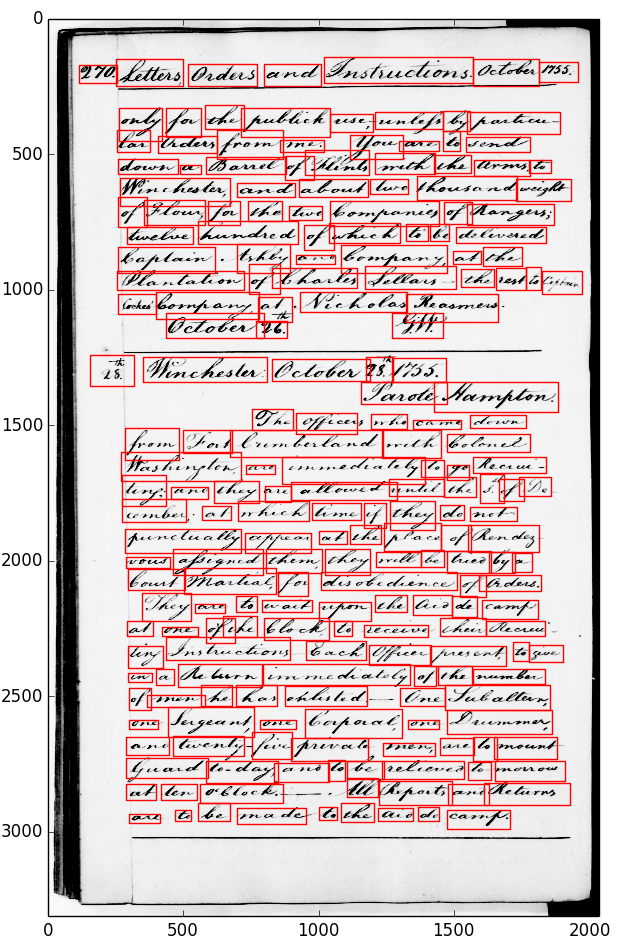
\includegraphics[scale=0.18]{Images/GT.png}
				\end{figure}
			\end{frame}
			
		\subsection{Inverted File Structure}
		
			\begin{frame}
				\frametitle{Inverted File Structure}
				\begin{figure}
					\centering
					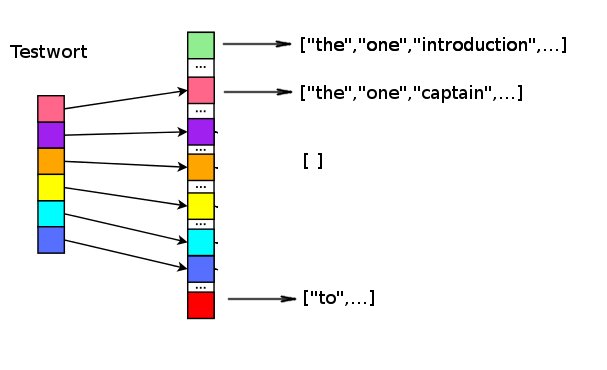
\includegraphics[scale=0.5]{Images/IFS.png}
				\end{figure}
			\end{frame}
			
		\subsection{Spatial Pyramid}
		
			\begin{frame}
				\frametitle{Spatial Pyramid}
				\begin{figure}
					\centering
					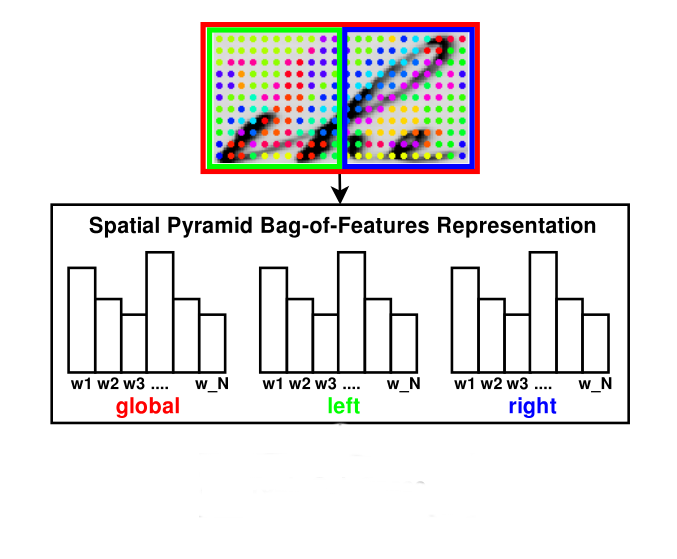
\includegraphics[scale=0.3]{Images/SpatialPyramids.png}
				\end{figure}
			\end{frame}
			
	\section{Ergebnisse}
		\subsection{Gütemaße}
			\begin{frame}
				\frametitle{Gütemaß}
				$
				\begin{array}{lcl}
					Precision & = & \frac{Ground\:Truth \:\cap\: Gefundene\:Woerter}{Gefundene\:Woerter}
				\end{array}
				$
				\\
				
			\end{frame}
			
		\subsection{Ergebnisse}
			\begin{frame}
				\frametitle{Stichproben}
				\begin{center}
					\begin{tabular}{|l|c|l|}
						\hline
						Wort & Erkennungsrate & Fehlerbeispiele\\
						\hline
						"to" & 85\% & "de", "be" \\
						\hline
						"immediately" & 100\% & ""\\
						\hline
						"october" & 67\% & "parole"\\
						\hline
						& & \\
						\hline
						"the" & 10\% & "be", "de", "are"\\
						\hline
						"be" & 8\% & "the", "de"\\
						\hline
						"of" & 10\% & "de", "a"\\
						\hline
					\end{tabular}
				\end{center}
			\end{frame}		
		
			\begin{frame}
				\frametitle{Gesamt}
				\begin{center}
					\begin{tabular}{|c|c|}
						\hline 
						Zellengröße & 5 \\ 
						\hline 
						Schrittgröße & 10 \\ 
						\hline 
						Zentroidenanzahl & 1000 \\ 
						\hline 
						Präzision & 30\% \\ 
						\hline 
					\end{tabular} 
				\end{center}
				
			\end{frame}
			
\end{document}
